\documentclass{article}
\usepackage[utf8]{inputenc}
\usepackage{amsmath}

\title{Iteracyjne metody rozwiązywania równań liniowych}
\author{Józef Jasek}

\usepackage{natbib}
\usepackage{graphicx}

\begin{document}

\maketitle

\section{Wstęp teoretyczny}
Omawiać będziemy 3 iteracyjne metody rozwiązywania układów postaci Ax = b, gdzie macierz A jest macierzą nieosobliwą, dominującą (warunek konieczny poprawności zastosowania poniższych metod), a x to macierz niewiadomych.
\subsection{Metoda Jacobiego}
Metoda ta polega na rozdzieleniu macierzy A na sumę dwóch macierzy - łatwo odwracalną macierz D zawierającą jedynie elementy na głównej przekątnej i R zawierającą pozostałe elementy (macierz tę można również podzielić na dwie macierze trójkątne, ale w praktyce nie będziemy dokonywać dzielenia na żadne macierze, gdyż jest to niepotrzebna i zasobożerna operacja). Wówczas rozwiązanie w danym kroku iteracyjnym wygląda następująco
\[ x_{k+1} = D^{-1}(b-Rx_k) \]
Możemy zauważyć, że udało się ograniczyć najbardziej czasochłonną część wyznaczania rozwiązania, czyli odwracanie macierzy do absolutnego minimum - macierz diagonalną można odwrócić w czasie liniowym, a przy zastosowaniu iteracji po poszczególnych x-ach tak naprawdę odbędzie się to w czasie stałym. Zatem każdy krok iteracji odbywa się w czasie $O(n^2)$ (mnożenie R i x).
\subsection{Metoda Gaussa-Seidela}
Metoda jest analogiczna do metody Jacobiego z tą różnicą, że w iteracji po poszczególnych $x^{k+1}_{i}$ korzystamy z tych x-ów które zostały już obliczone w obecnej iteracji. Intuicyjnie można to interpretować w następujący sposób: jeżeli każdy kolejny krok iteracji zbliża nas do rozwiązania, to $x^{k+1}_{j}$ jest bliżej prawdziwego rozwiązania niż $x^{k}_{j}$. Użycie go zatem powinno nas zbliżyć troszeczkę bardziej i troszeczkę szybciej do wyniku.
\subsection{Successive over-relaxation}
Jest to jeszcze szybsza modyfikacja metody Gaussa-Seidela. Wprowadza dodatkowy argument zwany parametrem relaksacji $\omega$
\[ 0 < \omega < 2 \]
Parametr $\omega$ wprowadza dodatkową zależność od $x^{k}$. Efekt może być dwojaki w zależności od tego jaki będzie znak $(1-\omega)$. Oznacza to albo opieranie się zmianom dla wartości większych od 0 albo wprost przeciwnie "uciekanie" od $x^{k}$. Istnieją metody pozwalające wyznaczyć optymalną wartość parametru, my decydujemy się jednak przyjąć jedną wartość.
\section{Pomiary szybkości zbiegania metod do rozwiązania}
Przyjmujemy $\omega = 1.2$. Wykonamy pomiary na 5 różnych równaniach. Wszystkie równania są postaci $Ax = b$. Na wykresach przedstawiono średnią różnicę pomiędzy elementami z macierzy $X_i$, która przedstawia rzeczywiste rozwiązania a wynikami otrzymanymi przez algorytm w kolejnych iteracjach. Przez $e_J$, $e_G$, $e_S$ oznaczymy średni błąd w 16 (ostatniej) iteracji dla metody odpowiednio Jacobiego, Gaussa-Seidela i SOR.
\[
A_0 =
\begin{bmatrix}
    4.0 & -1.0 & -0.2 & 2.0 \\
    -1.0 & 5.0 & 0.0 & -2.0 \\
    0.2 & 1.0 & 10.0 & -1.0 \\
    0.0 & -2.0 & -1.0 & -4.0 \\
\end{bmatrix}
B_0 = 
\begin{bmatrix}
    21.6 \\
    36 \\
    -20.6 \\
    -11\\
\end{bmatrix}
X_0 = 
\begin{bmatrix}
    7  \\
    9  \\
    -3 \\
    1  \\
\end{bmatrix}
\]
\noindent
\makebox[\textwidth]{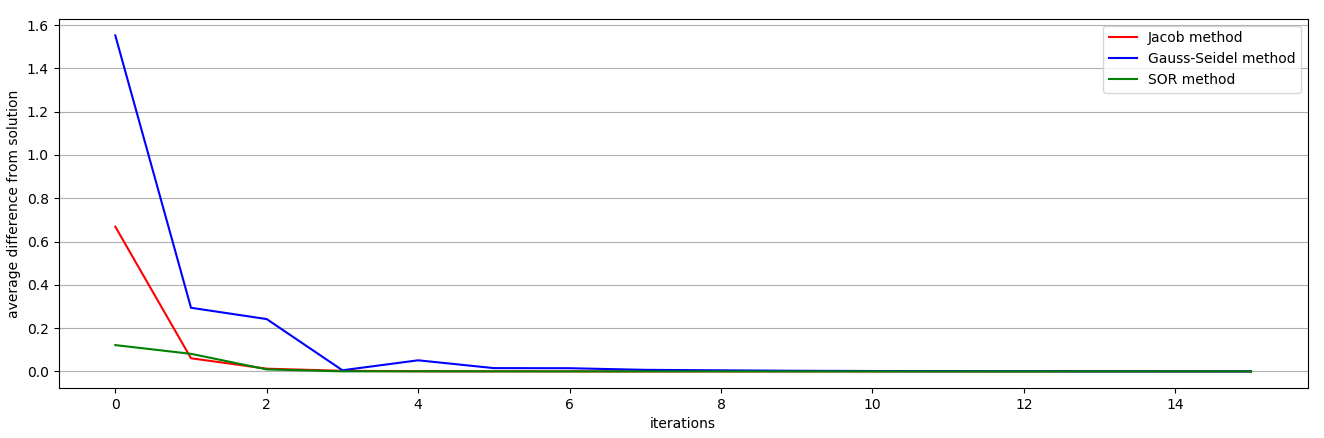
\includegraphics[width=1.7\textwidth]{0.png}}

\[ e_J = 2.335 \cdot 10^{-11} \]
\[ e_G = 1.51955 \cdot 10^{-4} \]
\[ e_S = 1.09655 \cdot 10^{-10} \]

\[
A_1 =
\begin{bmatrix}
    10.0 & -1.0 & 2.0 & 0.0 \\
    -1.0 & 11.0 & -1.0 &  3.0 \\
    2.0 & -1.0 & 10.0 & -1.0 \\
    0.0 &  3.0 & -1.0 &  8.0 \\
\end{bmatrix}
B_1 = 
\begin{bmatrix}
     6.0 \\
    25.0 \\
    -11.0 \\
    15 \\
\end{bmatrix}
X_1 = 
\begin{bmatrix}
    1.0  \\
    2.0  \\
    -1.0 \\
    1.0  \\
\end{bmatrix}
\]
\noindent
\makebox[\textwidth]{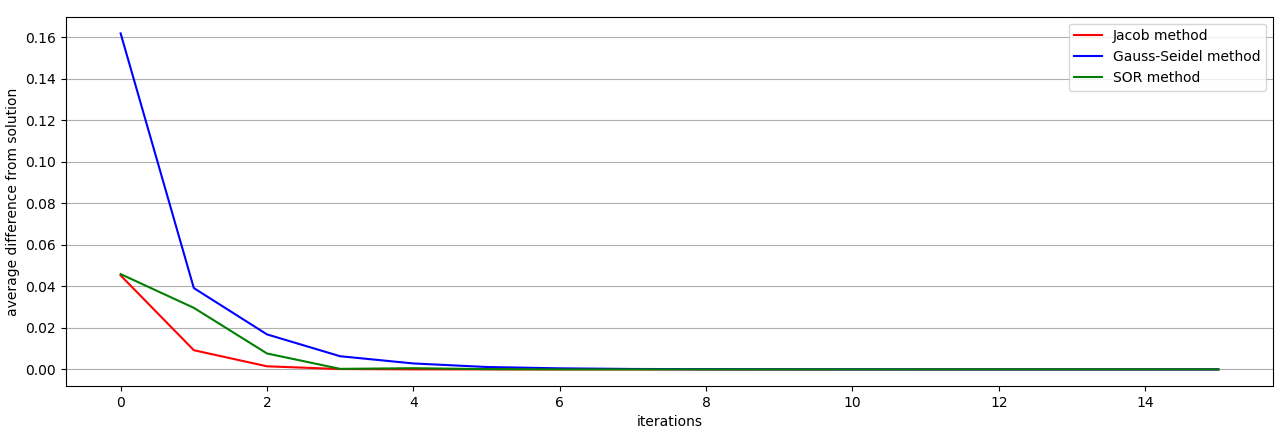
\includegraphics[width=1.7\textwidth]{1.png}}

\[ e_J = 8.32667 \cdot 10^{-17} \]
\[ e_G = 2.35383 \cdot 10^{-7} \]
\[ e_S = 9.75908 \cdot 10^{-12} \]

\[
A_2 =
\begin{bmatrix}
    1.0 & 0.0 & 0.0 \\
    0.0 & 1.0 & 0.0 \\
    0.0 & 0.0 & 1.0 \\
\end{bmatrix}
B_2 = 
\begin{bmatrix}
    1.0 \\
    1.0 \\
    1.0 \\
\end{bmatrix}
X_2 = 
\begin{bmatrix}
    1.0 \\
    1.0 \\
    1.0 \\
\end{bmatrix}
\]
\noindent
\makebox[\textwidth]{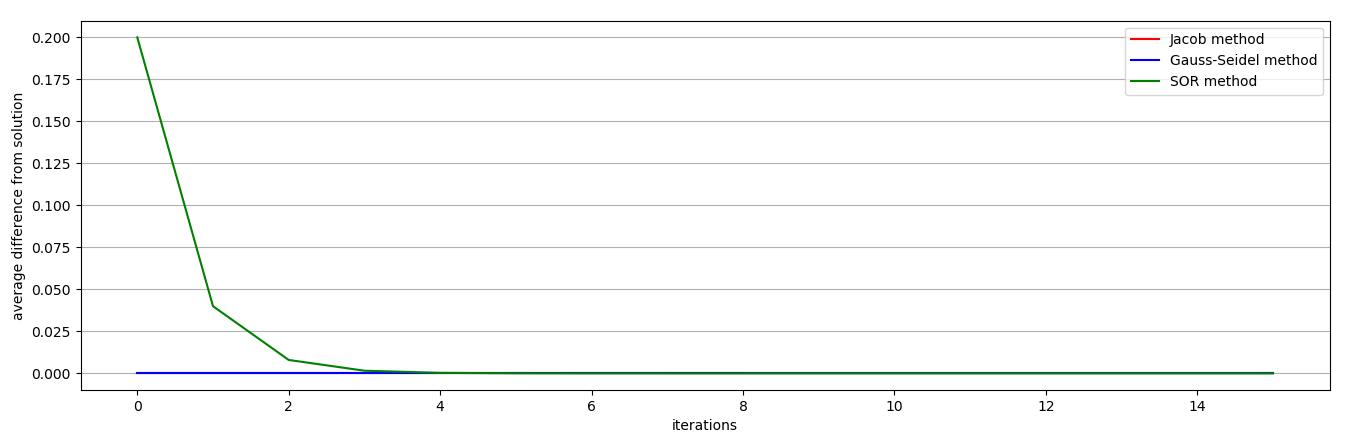
\includegraphics[width=1.7\textwidth]{2.png}}

\[ e_J = 0 \]
\[ e_G = 0 \]
\[ e_S = 6.55365 \cdot 10^{-12} \]

\[
A_3 =
\begin{bmatrix}
    1.0 & 0.0 & 0.0 \\
    0.0 & 1.0 & 0.0 \\
    0.0 & 0.0 & 1.0 \\
\end{bmatrix}
B_3 = 
\begin{bmatrix}
    0.0 \\
    0.0 \\
    0.0 \\
\end{bmatrix}
X_3 = 
\begin{bmatrix}
    0.0 \\
    0.0 \\
    0.0 \\
\end{bmatrix}
\]
\noindent
\makebox[\textwidth]{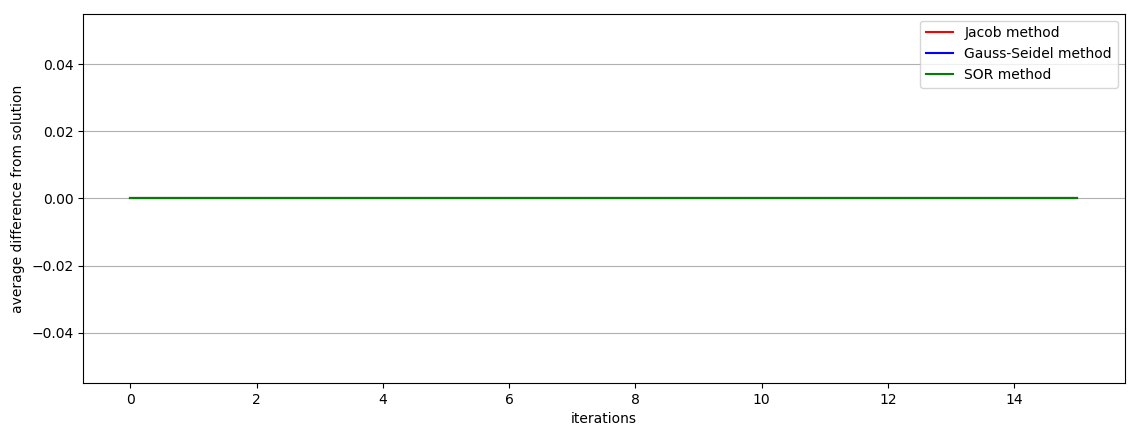
\includegraphics[width=1.7\textwidth]{3.png}}

\[ e_J = 0 \]
\[ e_G = 0 \]
\[ e_S = 0 \]

\[
A_4 =
\begin{bmatrix}
    990 &  71 &  678 & 443 &  67 \\
     45 & 867 &    1 & -23 &  42 \\
    213 & 123 & 7484 &   0 &   9 \\
     12 & 344 & -123 & 789 & -45 \\
     81 &  35 &   61 &  80 & 500 \\
\end{bmatrix}
B_4 = 
\begin{bmatrix}
    4899    \\
     821    \\
    -477055 \\
    19692   \\
    -9280   \\
\end{bmatrix}
X_4 = 
\begin{bmatrix}
    45  \\
     0  \\
    -65 \\
    13  \\
    -20 \\
\end{bmatrix}
\]
\noindent
\makebox[\textwidth]{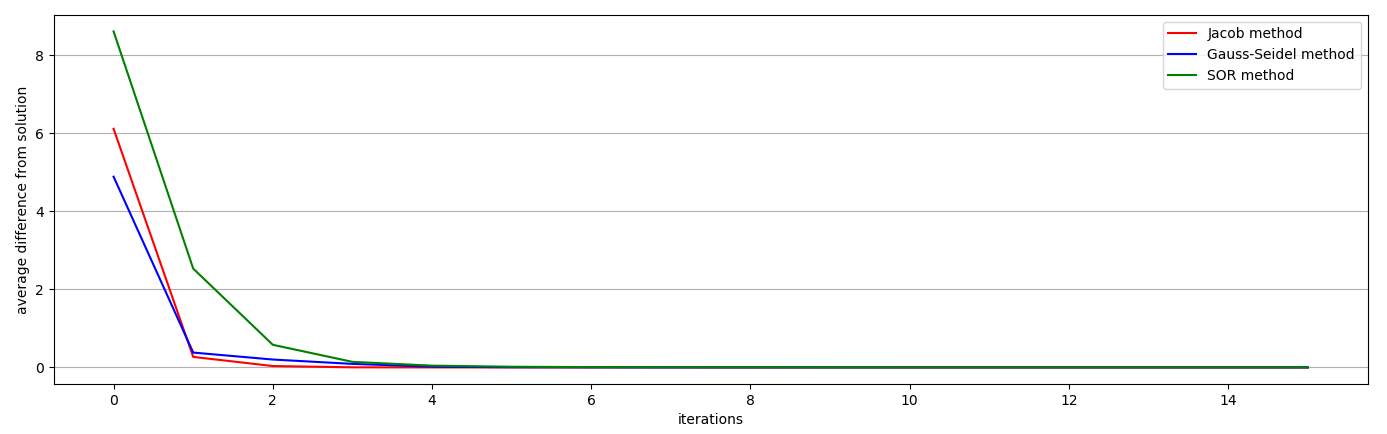
\includegraphics[width=1.7\textwidth]{4.png}}

\[ e_J = 2.62253 \cdot 10^{-17} \]
\[ e_G = 1.97575 \cdot 10^{-8} \]
\[ e_S = 1.28737 \cdot 10^{-6} \]
\section{Wnioski}
Co ciekawe najmniejszy błąd otrzymaliśmy dla metody Jacobiego. Szczególnie słaby wynik metody SOR, niezgodny z oczekiwaniami może wynikać ze źle dobranego parametru $\omega$ jak również z faktu, że rozwiązywano bardzo proste macierze, więc metoda nie mogła się "wykazać". 
\end{document}

